\section{$S^{n}$ 的基本群}
\label{section:ch09-sec59}

现在, 我们回到本章开头提到的问题, 即指出球面、环面、双环面从拓扑看来彼此不同的问题. 先来研究球面, 证明 $n\geqslant 2$ 时 $S^{n}$ 是单连通的. 我们需要以下重要的结论.

\par
\begin{figure}[htbp]
\centering
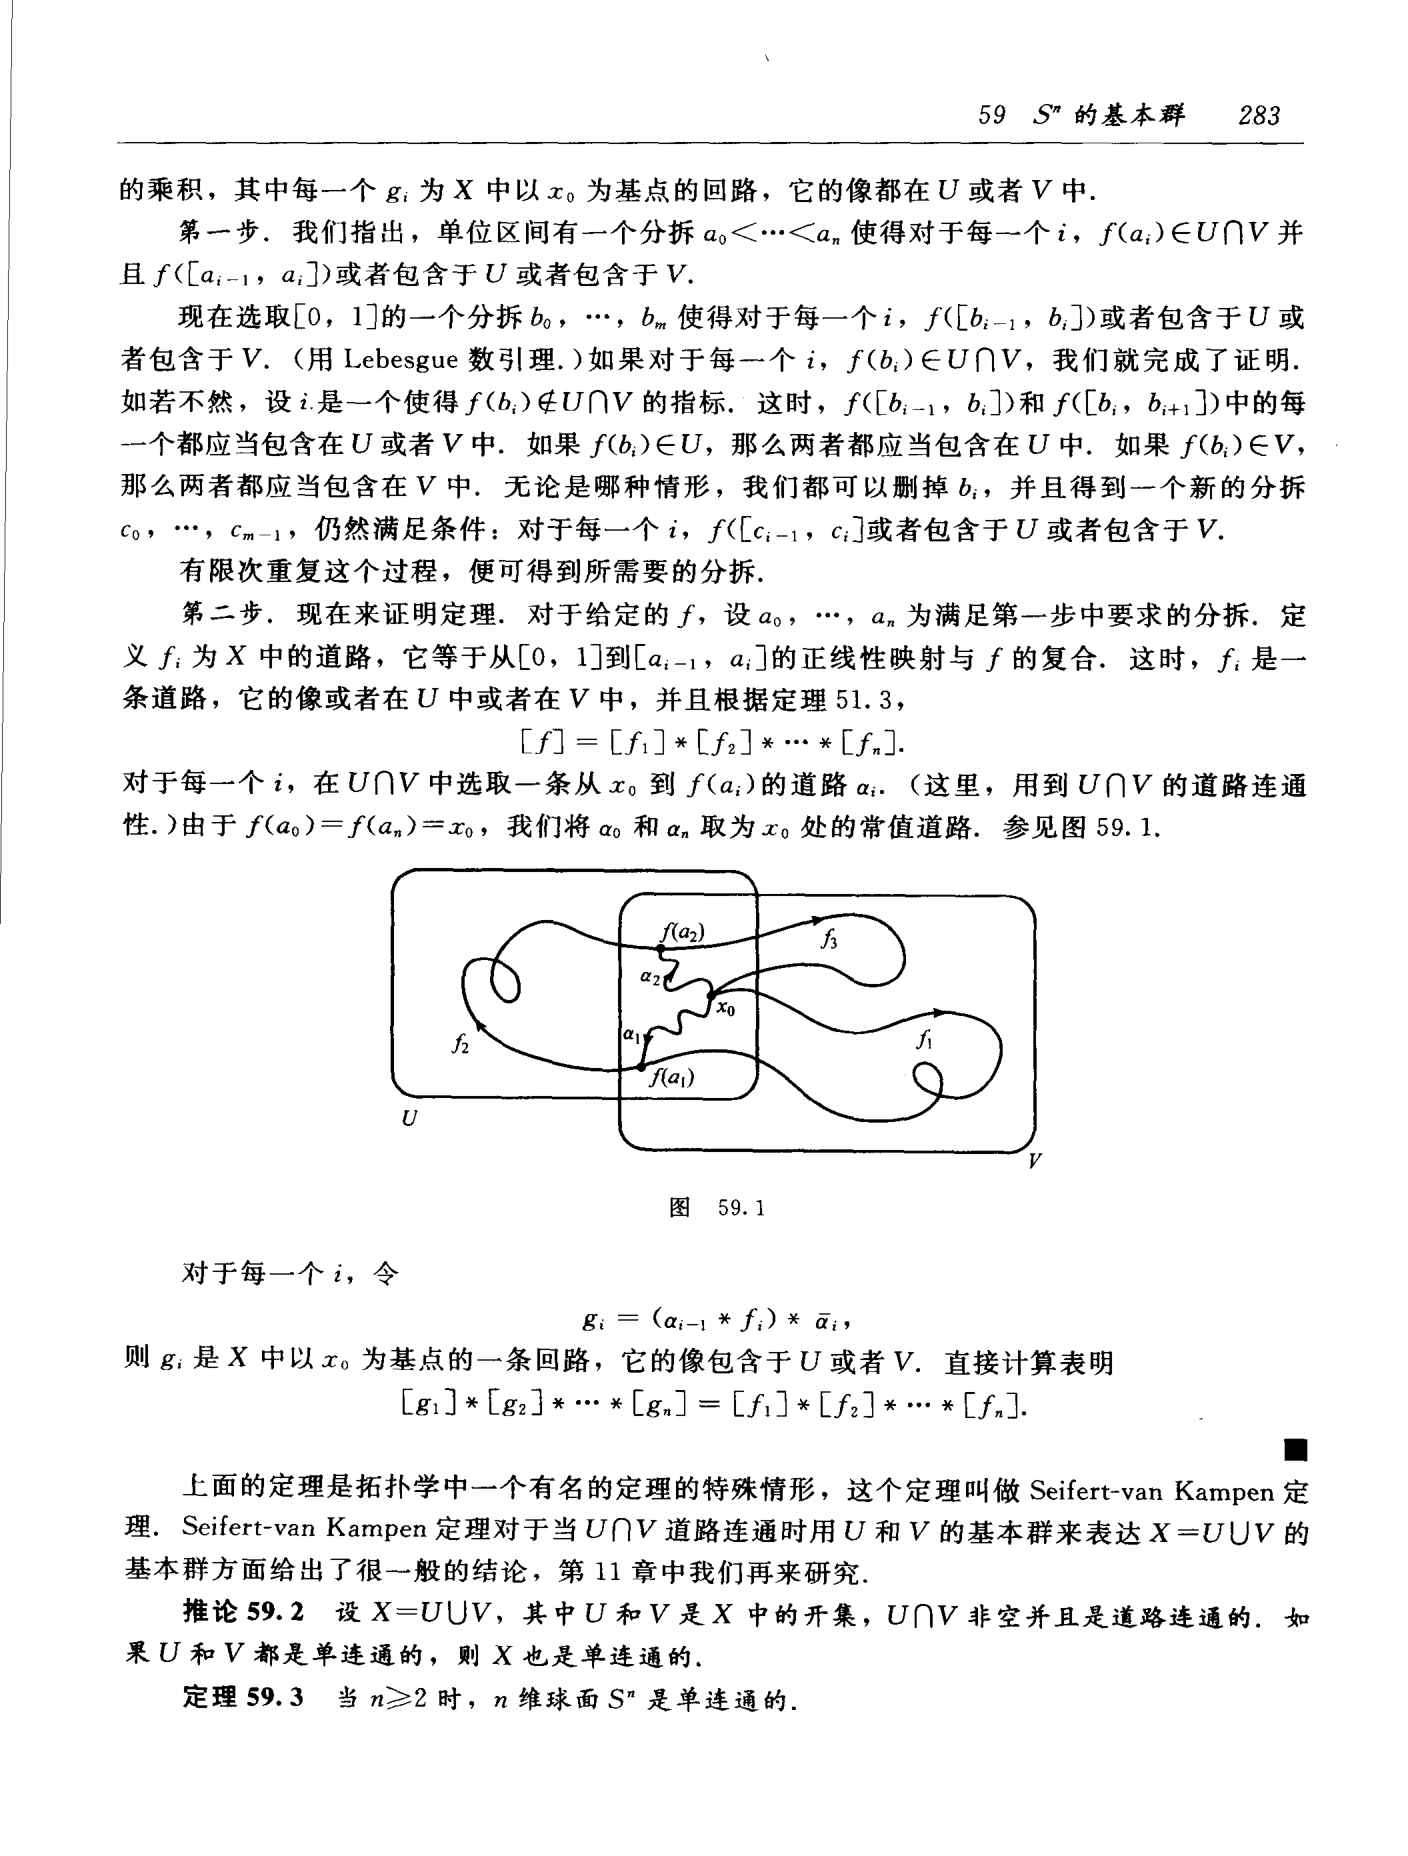
\includegraphics[width=0.6\textwidth]{image/fig-59-1.png}
\caption{定理 \cref{theorem:ch09-sec59-59-1} 的证明.}
\label{figure:ch09-fig-59-1}
\end{figure}

\begin{theorem}
\label{theorem:ch09-sec59-59-1}
设 $X=U\cup V$, 其中 $U$ 和 $V$ 是 $X$ 中的开集. 设 $U\cap V$ 是道路连通的, $x_0\in U\cap V$. 令 $i$ 和 $j$ 分别表示 $U$ 和 $V$ 到 $X$ 中的内射. 则诱导同态
\[
i_{*}\colon\pi_{1}(U,x_{0})\to\pi_{1}(X,x_{0})\quad\text{和}\quad
j_{*}\colon\pi_{1}(V,x_{0})\to\pi_{1}(X,x_{0})
\]
的像生成 $\pi_1(X,x_0)$.
\end{theorem}


\begin{proof}
这个定理是说, $X$ 中以 $x_0$ 为基点的任何回路都道路同伦于形如 $(g_1*(g_2*(\cdots*g_n)))$ 的乘积, 其中每一个 $g_i$ 为 $X$ 中以 $x_0$ 为基点的回路, 它的像都在 $U$ 或者 $V$ 中.

\textbf{第一步.} 我们指出, 单位区间有一个分拆 $a_0<\cdots<a_n$ 使得对于每一个 $i$, $f(a_i)\in U\cap V$ 并且 $f([a_{i-1},a_i])$ 或者包含于 $U$ 或者包含于 $V$.

现在选取 $[0,1]$ 的一个分拆 $b_0,\cdots,b_m$ 使得对于每一个 $i$, $f([b_{i-1},b_i])$ 或者包含于 $U$ 或者包含于 $V$. (用 Lebesgue 数引理.) 如果对于每一个 $i$, $f(b_i)\in U\cap V$, 我们就完成了证明. 如若不然, 设 $i$ 是一个使得 $f(b_i)\notin U\cap V$ 的指标. 这时, $f([b_{i-1},b_i])$ 和 $f([b_i,b_{i+1}])$ 中的每一个都应当包含在 $U$ 或者 $V$ 中. 如果 $f(b_i)\in U$, 那么两者都应当包含在 $U$ 中. 如果 $f(b_i)\in V$, 那么两者都应当包含在 $V$ 中. 无论是哪种情形, 我们都可以删掉 $b_i$, 并且得到一个新的分拆 $c_0,\cdots,c_{m-1}$, 仍然满足条件: 对于每一个 $i$, $f([c_{i-1},c_i])$ 或者包含于 $U$ 或者包含于 $V$.

有限次重复这个过程, 便可得到所需要的分拆.

\textbf{第二步.} 现在来证明定理. 对于给定的 $f$, 设 $a_0,\cdots,a_n$ 为满足第一步中要求的分拆. 定义 $f_i$ 为 $X$ 中的道路, 它等于从 $[0,1]$ 到 $[a_{i-1},a_i]$ 的正线性映射与 $f$ 的复合. 这时, $f_i$ 是一条道路, 它的像或者在 $U$ 中或者在 $V$ 中, 并且根据定理 \cref{theorem:ch09-sec51-51-3},
\[
[f]=[f_{1}]*[f_{2}]*\cdots*[f_{n}].
\]
对于每一个 $i$, 在 $U\cap V$ 中选取一条从 $x_0$ 到 $f(a_i)$ 的道路 $\alpha_i$. (这里, 用到 $U\cap V$ 的道路连通性.) 由于 $f(a_0)=f(a_n)=x_0$, 我们将 $\alpha_0$ 和 $\alpha_n$ 取为 $x_0$ 处的常值道路. 参见图 \cref{figure:ch09-fig-59-1}.


对于每一个 $i$, 令
\[
g_{i}=(\alpha_{i-1}*f_{i})*\bar{\alpha}_{i},
\]
则 $g_i$ 是 $X$ 中以 $x_0$ 为基点的一条回路, 它的像包含于 $U$ 或者 $V$. 直接计算表明
\[
[g_{1}]*[g_{2}]*\cdots*[g_{n}]=[f_{1}]*[f_{2}]*\cdots*[f_{n}].
\]
\end{proof}

上面的定理是拓扑学中一个有名的定理的特殊情形, 这个定理叫做 Seifert-van Kampen 定理. Seifert-van Kampen 定理对于当 $U\cap V$ 道路连通时用 $U$ 和 $V$ 的基本群来表达 $X=U\cup V$ 的基本群方面给出了很一般的结论, 第 11 章中我们再来研究.

\begin{corollary}
\label{corollary:ch09-sec59-59-2}
设 $X=U\cup V$, 其中 $U$ 和 $V$ 是 $X$ 中的开集, $U\cap V$ 非空并且是道路连通的. 如果 $U$ 和 $V$ 都是单连通的, 则 $X$ 也是单连通的.
\end{corollary}

\begin{theorem}
\label{theorem:ch09-sec59-59-3}
当 $n\geqslant 2$ 时, $n$ 维球面 $S^{n}$ 是单连通的.
\end{theorem}

\begin{proof}
令 $p=(0,\cdots,0,1)\in\mathbb{R}^{n+1}$ 和 $q=(0,\cdots,0,-1)$ 分别表示 $S^{n}$ 的"北极"和"南极".

\textbf{第一步.} 证明当 $n\geqslant 1$ 时, 穿孔球面 $S^{n}-p$ 同胚于 $\mathbb{R}^{n}$.

定义 $f\colon(S^{n}-p)\to\mathbb{R}^{n}$ 为
\[
f(x)=f(x_{1},\cdots,x_{n+1})=\frac{1}{1-x_{n+1}}(x_{1},\cdots,x_{n}).
\]
映射 $p$ 叫做\textbf{球极投射}(stereographic projection). ($\mathbb{R}^{n+1}$ 中通过北极 $p$ 和 $S^{n}-p$ 上的点 $x$ 的直线与 $n$ 维平面 $\mathbb{R}^{n}\times 0\subset\mathbb{R}^{n+1}$ 交于点 $f(x)\times 0$.) 为了验证 $f$ 是一个同胚, 定义映射 $g\colon\mathbb{R}^{n}\to(S^{n}-p)$ 使得
\[
g(y)=g(y_{1},\cdots,y_{n})=(t(y)\cdot y_{1},\cdots,t(y)\cdot y_{n},1-t(y)),
\]
其中 $t(y)=2/(1+\|y\|^{2})$. 我们只要验证 $g$ 既是 $f$ 的左逆也是 $f$ 的右逆就可以了.

反射 $(x_1,\cdots,x_{n+1})\mapsto(x_1,\cdots,x_n,-x_{n+1})$ 是 $S^{n}-p$ 到 $S^{n}-q$ 的一个同胚, 所以 $S^{n}-q$ 也同胚于 $\mathbb{R}^{n}$.

\textbf{第二步.} 现在来证明定理. 设 $U=S^{n}-p$ 和 $V=S^{n}-q$, 它们都是 $S^{n}$ 中的开集.

首先注意, 当 $n\geqslant 1$ 时, 球面 $S^{n}$ 是道路连通的. 这是因为 $U$ 和 $V$ 都是道路连通的 (它们都同胚于 $\mathbb{R}^{n}$), 并且有一个公共点 $(1,0,\cdots,0)$.

现在证明: 当 $n\geqslant 2$ 时, 球面 $S^{n}$ 是单连通的. 空间 $U$ 和 $V$ 都是单连通的, 因为它们同胚于 $\mathbb{R}^{n}$. $U$ 和 $V$ 的交等于 $S^{n}-p-q$, 在球极投射下同胚于 $\mathbb{R}^{n}-\boldsymbol{0}$. 这个空间是道路连通的, 因为 $\mathbb{R}^{n}-\boldsymbol{0}$ 中的每一个点都可以用直线连接到 $S^{n-1}$ 的一个点, 而当 $n\geqslant 2$ 时, $S^{n-1}$ 是道路连通的. 于是应用前面的推论便可完成定理的证明.
\end{proof}

\subsection*{习题}

\begin{exercise}
设 $X$ 是 $S^{2}$ 的两个交于一点的副本之并. $X$ 的基本群是什么? 证明你的结论. [小心! 交于一点的两个单连通空间之并可以不是单连通的. 参见 [S], p. 59.]
\end{exercise}

\begin{exercise}
对以下 $S^{2}$ 的单连通性的"证明"加以批评: 设 $f$ 是 $S^{2}$ 中以 $x_0$ 为基点的回路. 在 $S^{2}$ 中选取一个不在 $f$ 的像中的点 $p$. 由于 $S^{2}-p$ 同胚于 $\mathbb{R}^{2}$, 而 $\mathbb{R}^{2}$ 是单连通的, 所以回路 $f$ 道路同伦于常值道路.
\end{exercise}

\begin{exercise}
(a) 证明当 $n>1$ 时, $\mathbb{R}^{1}$ 与 $\mathbb{R}^{n}$ 不同胚.
(b) 证明当 $n>2$ 时, $\mathbb{R}^{2}$ 与 $\mathbb{R}^{n}$ 不同胚.

事实上, 当 $n\neq m$ 时, $\mathbb{R}^{n}$ 和 $\mathbb{R}^{m}$ 不同胚, 但其证明要用到更多代数拓扑的工具.
\end{exercise}

\begin{exercise}
同定理 \cref{theorem:ch09-sec59-59-1} 的假设.
(a) 如果 $j_*$ 是平凡的同态, 或者 $i_*$ 和 $j_*$ 都是平凡的同态, 你能对 $X$ 的基本群给出什么结论?
(b) 给出一个例子, 使得 $i_*$ 和 $j_*$ 都是平凡的, 但 $U$ 和 $V$ 的基本群都不是平凡的.
\end{exercise}